% !TEX root = Ausarbeitung.tex


\section{Einleitung}
\subsection{Projektbeschreibung}
Im Januar 2020 wird in den USA ein Gesetz in Kraft treten. Dieses verpflichtet die Firma T dazu, alle Schiffscontainer mit einem Tracking-Gerät auszustatten. Dieses Gerät muss die Position des entsprechenden Container über die letzten 9 Monate dokumentieren. Unsere Geräte CONTRAC mit der zugehörigen Software CONSERV bietet diese Möglichkeit. Aus diesem Grund hat uns KT beauftragt die Container des Schiffs "`Event Horizon"' mit unserem System auszustatten. Um die Anforderungen der Firma KT zu erfüllen müssen diese Geräte allerdings mit ZigBee ausgestattet werden und die Software entsprechend erweitert werden. Auch übernehmen wir die Verwaltung des Servers CONSERV für KT.
\section{Annahmen}
\subsection{Sitze und Örtlichkeiten}
\begin{enumerate}
    \item Der Sitz der Firma EZ ist Albstadt
    \item Der Sitz der Firma DOTDAT GmbH ist Hamburg
    \item Der bei KT beschäftigte Projektleiter Lars Haekinson arbeitet in Hamburg
    \item Die Firma EZ besitzt einen Vorrat von ca. 100 CONTRAC-Geräten für Test- und Entwicklungszwecke in Albstadt
    \item Der Kunde verlangt keine Änderungen während des Projektzeitraums
   
    \item Die Kosten für die CONTRACK-Geräte enthalten eine Pauschale für eine LTE Verbindung mit einer eingebaut E-Sim.
	\item Die Tochterfirma kann jederzeit, ohne Verzögerungen mit der Produktion beginnen.
    \item Die Lieferung großer Frachten aus Shenzhen dauert 40 Tage und kostet 1.500 Euro pro Container.
    \item Die Lieferung kleiner Mengen per Luftfracht dauert 5 Tage und kostent 20.000 pro Tonne.
    \item Alle Mitarbeiter sind in der angegebenen Zeit für das Projekt verfügbar.
\end{enumerate}

\section{Projektinhalt}
\subsection{Aktivitäten}
\begin{table}[H]
    \renewcommand{\arraystretch}{1.05}
    \begin{center}
        \begin{tabular}{l|l}
            \hline
            \textbf{ID} & \textbf{Aktivität}\\\hline
            % Planung nicht teil des Projektplan
            A    & Projektmanager                                      \\ \hline
            A1   & Ausführungen                                        \\ \hline
            A2   & Reviews                                             \\ \hline
            A3 & Kommunikation \\\hline
            B    & CONTRAC                                             \\ \hline
            B1   & Entwicklung Verbesserung Hardware (ZigBee und Akku) \\ \hline
            B2.X & Einkauf der Teile\\\hline
            B2.1 & Produktion beauftragen                              \\ \hline
            B2.2 & Produktion                                          \\ \hline
            B3.1 & QS Shenzhen                                         \\ \hline
            % Versand nicht als Aktivität
            B4.1 & Versand                                             \\ \hline
            B3.2 & QS Hamburg                                          \\ \hline
            B4.2 & Versand Rotterdam                                   \\ \hline
            B5.1 & Anbauer Suchen                                      \\ \hline
            B5.2 & Anbau entwerfen                                     \\ \hline
            B5.3 & Anbau testen                                        \\ \hline
            B5.4 & Anbau vorstellen                                    \\ \hline
            B5.5 & Anbau verbessern                                    \\ \hline
            B5.6 & Anbauteile bestellen                                \\ \hline
            B5.7 & Anbau                                               \\ \hline
            C    & CONSERV                                             \\ \hline
            C1.1 & Patch-Software optimieren                           \\ \hline
            C1.2 & Patch-Software testen                               \\ \hline
            C1.3 & Patch-Software Fehler beheben                       \\ \hline
            C2   & Mit 5500 Geräten testen                             \\ \hline
            C3.1 & Cloud-Anbieter suchen                               \\ \hline
            C3.2 & Angebote einholen                                   \\ \hline
            C3.3 & Cloud einrichten                                    \\ \hline
            C3.4 & Server einrichten                                   \\ \hline
            D    & CONTRAC-Firmware                                    \\ \hline
            D1   & ZigBee einbauen                                     \\ \hline
            D2.1 & Patch-Funktion optimieren                           \\ \hline
            D2.2 & Patch-Funktion testen                               \\ \hline
            D2.3 & Patch-Funktion Fehler beheben                       \\
        \end{tabular}
        \caption{Aktivitäten im Projekt}
    \end{center}
\end{table}

\subsection{Work-Breakdown-Strukture}
\begin{figure}[H]
    \begin{center}
        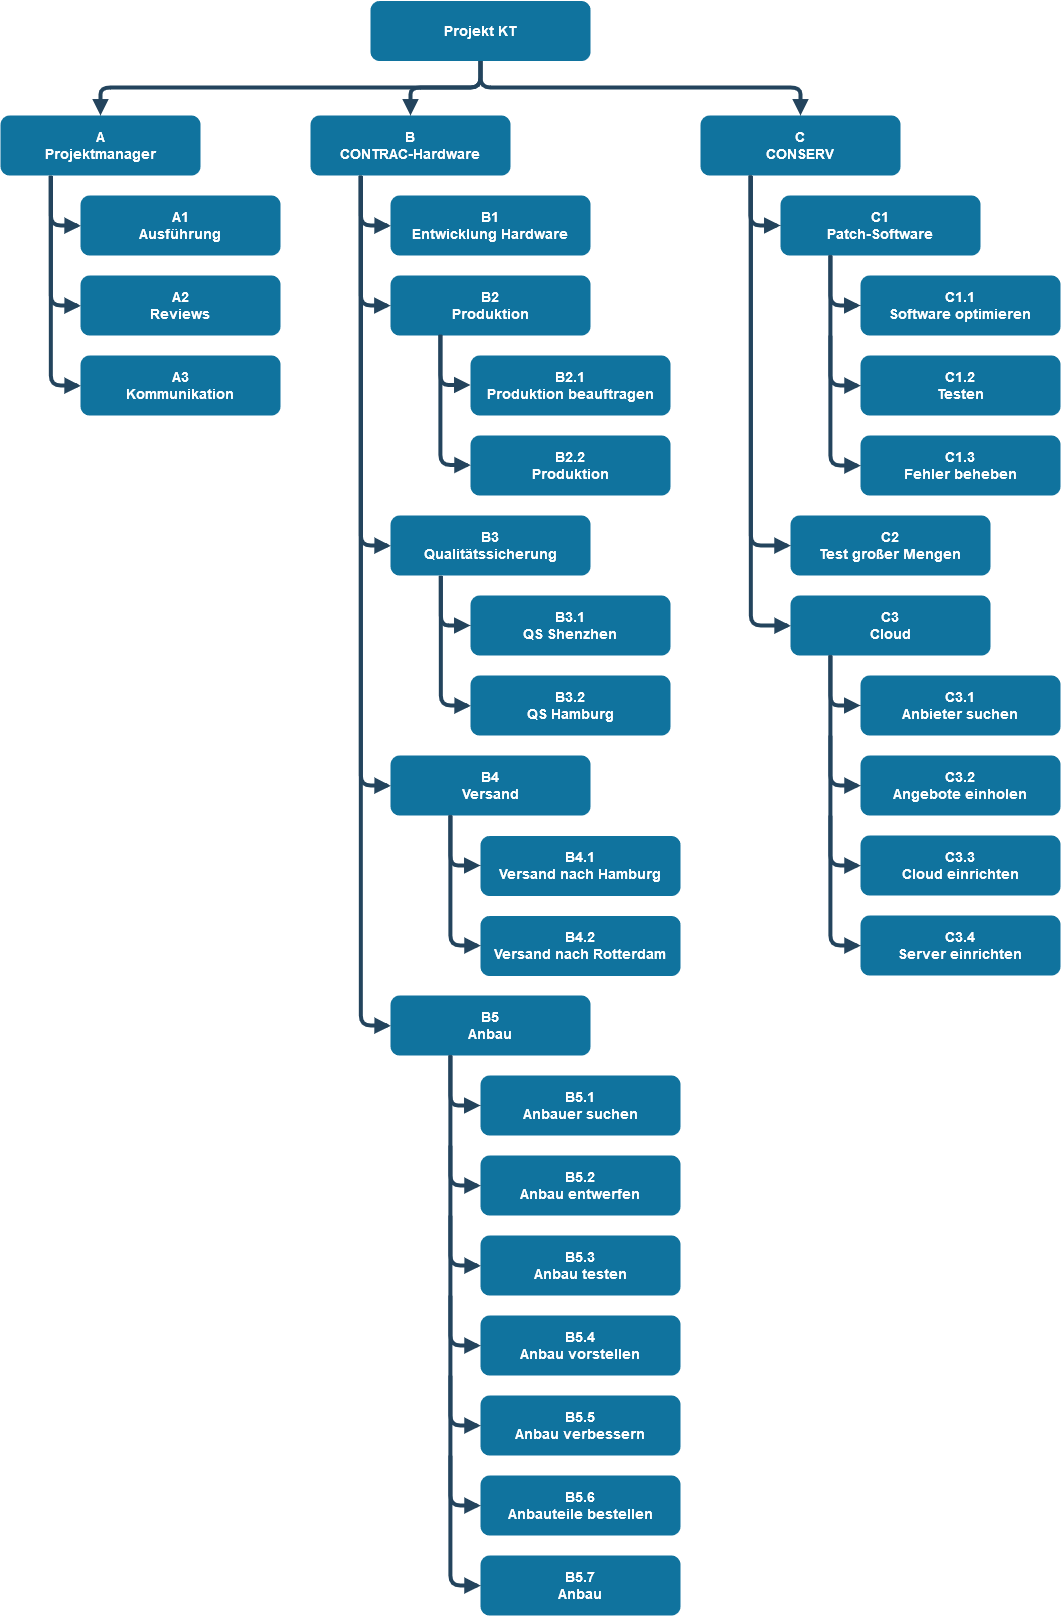
\includegraphics[width=0.8\textwidth]{WBS.png}
    \end{center}
    \caption{Work-Breakdown-Strukture}
\end{figure}
\subsection{Oranisation Breakdown Strukture}
\begin{figure}[H]
    \begin{center}
        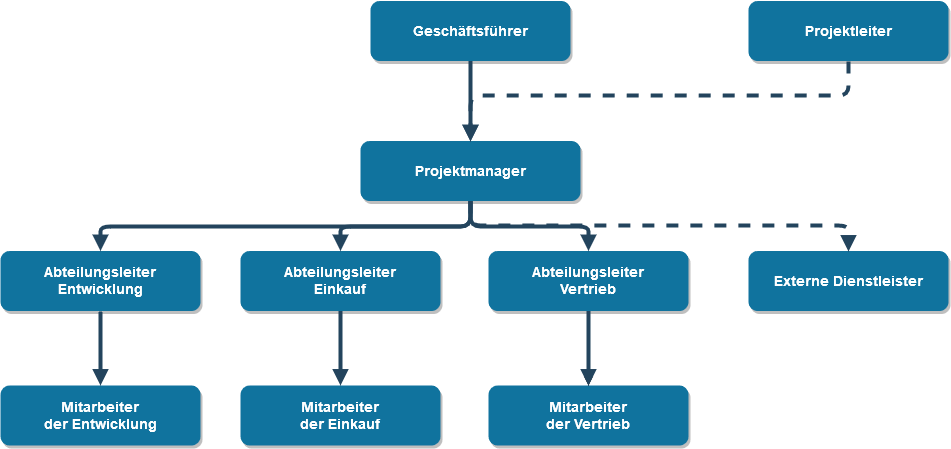
\includegraphics[width=0.8\textwidth]{OBS.png}
    \end{center}
    \caption{Organisation-Breakdown-Strukture}
\end{figure}
\section{Zeitmanagement}
\subsection{Aktivitätendauer}


\subsection{Meilensteine}

\paragraph{M1: Patch-Update Funktion funktionstüchtig} Die Patch-Update Funktion wurde erfolgreich getestet und die dementsprechende Entwicklung ist abgeschlossen.
\paragraph{M2: CONTRACK-Firmware um ZigBee ergänzt} Die Firmware für die CONTRACK-Geräte wurde für ZigBee ergänzt und erfolgreich getestet.
\paragraph{M3: Hardeware-Entwicklung abgeschlossen} Die Entwicklung der Hardware mit den Ergänzungen um ZigBee und größeren Akku ist abgeschlossen.
\paragraph{M4: Produktion in Shenzhen beauftragt} Die Produktion der Geräte in Shenzhen wurde in Auftrag gegeben.
\paragraph{M5: CONSERV-Server mit 5250 Geräten getestet} Der CONSERV-Server wurde mit 5250 erfolgreich getestet.
\paragraph{M6: QS Shenzhen erfolgreich} Alle produzierten Geräte haben die Qualiätssicherung in Shenzhen erfolgreich bestanden.
\paragraph{M7: Geräte aus Shenzhen empfangen} Die Geräte aus Shenzhen sind unbschadet in Rotterdam angekommen.
\paragraph{M8: Montage von KT abgenommen} Der Montagevorgang wurde von KT abgenommen.
\paragraph{M9: Geräte montiert} Die Geräte wurden alle an den Containern montiert.
\paragraph{M10: Inbetriebnahme} Alle Geräte wurden problemlos in Betrieb genommen.




\subsection{PERT} % Kritischer Pfad !

\subsection{Gant} % Kritischer Pfad !

\section{Kommunikationsplan}
\subsection{Stakeholder}
\begin{table}[H]
    \renewcommand{\arraystretch}{1.1}
    \begin{center}
        \begin{tabular}{l|l}
            \textbf{Stakeholder} & \textbf{Kürzel}\\\hline
            
            
            
            
        \end{tabular}
    \end{center}
    \caption{Stakeholder}
\end{table}
\subsection{Regelmeetings}
 
\subsubsection{Kickoff}
\textbf{Wann:} 
\textbf{Wer:}
\textbf{Wo:}
\textbf{Wie oft:}
\textbf{Produzierte Dokumente:}


\subsubsection{Dayly}
\textbf{Wann:} 
\textbf{Wer:}
\textbf{Wo:}
\textbf{Wie oft:}
\textbf{Produzierte Dokumente:}

\subsubsection{Weekly Review}
\textbf{Wann:} 
\textbf{Wer:}
\textbf{Wo:}
\textbf{Wie oft:}
\textbf{Produzierte Dokumente:}

\subsubsection{Präsentation der Befestigung}
\textbf{Wann:} 
\textbf{Wer:}
\textbf{Wo:}
\textbf{Wie oft:}
\textbf{Produzierte Dokumente:}

\subsection{Statusberichte}
Sämtliche Berichte werden im firmeneigenen Confluence gesammelt und allen Beteiligten zur Verfügung gestellt.

\subsubsection{Template für Statusberichte}


\section{Qualität}
\subsection{Qualitätsprozesse}
Um die Qualität der Hardware und Software werden bei EZ verschieden Prozesse eingesetzt. Dazu gehört eine doppelte Qualitätskontrolle der Hardware, Code Reviews sowie ausführliche und automatisierte Tests für die Software.
\subsection{Qualitätskontrolle der Hardware}
Alle CONTRAC-Geräte werden in Shenzhen und in Hamburg durch eine elektrische Kontrolle auf ihre Funktionalität geprüft.
\subsubsection{Code Review}
Jeder Code muss vor dem Mergen in den master-Branch durch einen zweiten Entwickler getestet und kontrolliert werden.
\subsubsection{Unit Test}
Für jede Softwarekomponente muss ein Unit-Test erstellt werden, der vor jedem Einchecken erfolgreich durchgeführt werden muss. Auch der Build-Server des Continuous-Integration-Zyklus muss die Tests erfolgreich ausführen. Bei einem Fehlschlag muss dieser zeitnah behoben werden.
\subsubsection{Test}
Jede erstellte Komponente muss vom Entwickler ausführlich getestet werden. Jede Komponente muss auch von einem zweiten Mitarbeiter getestet werden.
\subsection{Ticketsytem}
Als Ticktsystem kommt das firmeneigene Jira zum Einsatz. Dieses ist über die Adresse \texttt{https://jira.ez.de} verfügbar. Alle Entwickler und Product Owner besitzen ein Zugang zu diesem System.
\subsection{Versionierungssystem}
Als Versionierungssystem für das Projekt wird Git eingesetzt. Dieses ist allen Entwicklern auf ihren Computern verfügbar. Als Git-Remote dient der firmeneigene Bitbucket-Server, der unter der Adresse \texttt{git.ez.de} verfügbar ist. Auch aus dem Internet ist der Server unter dieser Adresse verfügbar.

Eine Commit-Message muss immer die getätigte Arbeit beschreiben und eine eindeutige Zuordung zu einem Ticket oder ein User Story ermöglichen. Dazu werden diese über ihre eindeutige Bezeichnung (US-3, BUG-5) erwähnt.
\subsection{Codestyle}
Der geschriebene Code muss den Stylerichtlinien der Firma entsprechen. Diese können dem hausinternen Wiki unter \texttt{wiki.ez.de} entnommen werden. Konfigurationsdateien für verschiedene IDEs und Formatierer können dort auch heruntergeladen werden. Diese Richtlinien werden auch an externe Firmen weitergegeben. 
\subsection{Bugverlauf}
Jeder entdeckte Bug muss in Jira dokumentiert werden. Die Bugs fließen dann in die Backlogs für die Entwicklung ein. Dort werden sie mit erhöhter Priorität belegt.


\subsection{Befestigung des Gerät CONTRACK}
Das Gerät CONTRACK muss am 15. Oktober innerhalb von 72h an 5000 Containern befestigt werden.

Die Geräte werden an den Containern mit Spezialkleber befestigt. Der Kleber wird von der Firma Sika hergestellt und regulär für das Verkleben von Fahrzeugkarosserien verwendet. Er wir dort als Ersatz von Schweißnähten genutzt und hält großen Belastungen und Temperaturschwankungen stand.\\
Die Montage wird von Zweierteams durchgeführt. Dieses reinigt zuerst mit einem sich verflüchtigendem Reinigungsmittel die Montagestelle am Container. Dann wird ein CONTRACK-Geräte in das Aufpresswerkzeug gesetzt. Der Kleber wird mit einer Spritze aufgetragen, das Gerät an den Container angepresst und anschließend angeschaltet. Dieser Vorgang kann in 2 Minuten durchgeführt werden. Die Arbeiter stehen für die Montage auf einer erhöhten Fläche, um den Montagepunkt leichter zu erreichen. Das Aufpresswerkzeug besitzt wie ein Drehmomentschlüssel einen Auslösemechanismus um den optimalen Druck zu gewährleisten.

Für die Montage in Rotterdam werden externe Mitarbeiter akquiriert, die diese Arbeit unter Aufsicht durchführen. Diese werden am Tag vor der Montage geschult. Die Montage findet an 6 Containerbrücken statt. Da für die Verladung eines Containers ca. 3,2\,min benötigt werden, dauert die Montage entsprechend 45 Stunden. In dieser Zeit wechseln sich Zweierteams im Dreischichtbetrieb ab. Damit sind für die Montage 36 Arbeiter notwendig.


\section{Risikoplan}
\subsection{Annahmen} % Auswahl

\subsubsection{Änderungen während der Projektlaufzeit}

\subsubsection{Verzögerung der Produktion}

\subsubsection{Die Lieferung der Geräte schlägt fehl}

\subsection{Risiken mit Priorität} %3 Stück

Die drei wichtigsten Risiken sind die folgenden:
\begin{enumerate}
	\item R1: Änderungen während der Projektlaufzeit
	\item R2: Verlust der Geräte bei Versand
	\item R3: Unerwarteter Mitarbeiterausfall
\end{enumerate}


\subsection{Bewertung } %Wahrscheinlichkeitsanalyse, Risikomatrix
Die Bewertung des Schadens wird wie folgt gestaffelt:	


Daraus lässt sich die folgende Risikomatrix abbilden:


\subsubsection{R1: Änderungen während der Projektlaufzeit}

\subsubsection{R2: Verlust der Geräte bei Versand}
\begin{enumerate}
	\item \textbf{Schaden}:
		\item \textbf{Schaden}:
			\item \textbf{Wahrscheinlichkeit}:
				\item \textbf{Klassifizierung}:
					\item \textbf{Gegenmaßnahmen}:
\end{enumerate}
\subsubsection{R3: Unerwarteter Mitarbeiterausfall}
\paragraph{Wahrscheinlichkeitsanalyse}

\subsection{Risikokosten}

Die Kosten für die Risiken betragen sich damit auf:



\section{Human Ressources}
\subsection{Aufgabenverteilung}
\begin{table}[H]
    \renewcommand{\arraystretch}{1.1}
    \begin{center}
        \begin{tabular}{l|l}
            \hline
            A    & Projektmanager                                      \\ \hline
            A1   & Ausführungen                                        \\ \hline
            A2   & Reviews                                             \\ \hline
            A3 & Kommunikation \\\hline
            &                                                   \\ \hline
            B    & CONTRAC                                             \\ \hline
            B1   & Entwicklung Verbesserung Hardware (ZigBee und Akku) \\ \hline
            B2.1 & Produktion beauftragen                              \\ \hline
            B2.2 & Produktion                                          \\ \hline
            B3.1 & QS Shenzhen                                         \\ \hline
            B4.1 & Versand                                             \\ \hline
            B3.2 & QS Hamburg                                          \\ \hline
            B4.2 & Versand Rotterdam                                   \\ \hline
            B5.1 & Anbauer Suchen                                      \\ \hline
            B5.2 & Anbau entwerfen                                     \\ \hline
            B5.3 & Anbau testen                                        \\ \hline
            B5.4 & Anbau vorstellen                                    \\ \hline
            B5.5 & Anbau verbessern                                    \\ \hline
            B5.6 & Anbauteile bestellen                                \\ \hline
            B5.7 & Anbau                                               \\ \hline
            &                                                     \\ \hline
            C    & CONSERV                                             \\ \hline
            C1.1 & Patch-Software optimieren                           \\ \hline
            C1.2 & Patch-Software testen                               \\ \hline
            C1.3 & Patch-Software Fehler beheben                       \\ \hline
            C2   & Mit 5500 Geräten testen                             \\ \hline
            C3.1 & Cloud-Anbieter suchen                               \\ \hline
            C3.2 & Angebote einholen                                   \\ \hline
            C3.3 & Cloud einrichten                                    \\ \hline
            C3.4 & Server einrichten                                   \\ \hline
            &                                                     \\ \hline
            D    & CONTRAC-Firmware                                    \\ \hline
            D1   & ZigBee einbauen                                     \\ \hline
            D2.1 & Patch-Funktion optimieren                           \\ \hline
            D2.2 & Patch-Funktion testen                               \\ \hline
            D2.3 & Patch-Funktion Fehler beheben                       \\
        \end{tabular}
        \caption{Aufgabenverteilung im Projekt}
    \end{center}
\end{table}
\subsection{Aktionsplan}



\subsection{Motivation} % Teamevents, Awards .. (kostet Geld)



\section{Beschaffung} % UserStories an extenern Firma
Bei der Firma DOTDAT GmbH wird die Entwicklung der Hardware eingekauft. Die von DOTDAT angefragten UserStories lauten wie folgt:

% Gerät bei Tochterfirma

% Material für Anbau

% Helfer für Anbau

% Cloudpartner

% 

% Softwarelizenzen



\section{Kostenmanagement}



\subsection{Kostenschätzung}
\lipsum[2]
\subsection{Personalkosten} % Awards, Reise, Hotel, Betriebssätze ...
\lipsum[2]
\subsection{Materialkosten}
\lipsum[2]
\subsection{Risikokosten}
\lipsum[2]
\subsection{Gewinnmarge}
\lipsum[2]
\subsection{Kontigenz} %
\lipsum[2]
\subsection{Plankosten}
\lipsum[2]





